\documentclass[12pt, letterpaper]{article}
\usepackage{graphicx} % Required for inserting images
\usepackage{hyperref}
\usepackage{listings}
\usepackage{amssymb}
\usepackage{amsmath}
\usepackage[english]{babel}
\usepackage{nicefrac, xfrac}
\usepackage{mathtools}
\newcommand{\acc}{\\\hphantom{}\\}
\usepackage[table,xcdraw]{xcolor}
\usepackage[paper=a4paper,left=20mm,right=20mm,bottom=25mm,top=25mm]{geometry}
\renewcommand{\labelenumii}{\arabic{enumi}.\arabic{enumii}}
    \renewcommand{\labelenumiii}{\arabic{enumi}.\arabic{enumii}.\arabic{enumiii}}
    \renewcommand{\labelenumiv}{\arabic{enumi}.\arabic{enumii}.\arabic{enumiii}.\arabic{enumiv}}
\title{Università 1 (gruppo 42)}
% \author{ Giacomo Biribicchi \and Marco Casu \and Christian Di Manno \and Alessandro Gautieri }
\date{}


\begin{document}

\maketitle


\section{Requisiti}
I dati di interesse per il sistema sono \underline{Studenti}, \underline{Facoltà}, \underline{Professori} e \underline{Corsi}.
\begin{enumerate}
    \item \textbf{Studente}\begin{enumerate}
        \item nome e cognome
        \item codice fiscale 
        \item matricola 
        \item data di nascita 
        \item città di nascita 
        \item corso di laurea 
        \item esami superati
    \end{enumerate}
    \item \textbf{Professore}\begin{enumerate}
        \item nome e cognome
        \item data di nascita 
        \item codice fiscale 
        \item città di nascita 
        \item insegnamenti erogati
    \end{enumerate}
    \item \textbf{Corso di Laurea}\begin{enumerate}
        \item nome 
        \item facoltà
    \end{enumerate}
    \item \textbf{Facoltà}\begin{enumerate}
        \item nome
    \end{enumerate}
    \item \textbf{Insegnamento}\begin{enumerate}
        \item nome 
        \item ore di lezione 
        \item corsi alla quale appartiene
        \item codice
    \end{enumerate}
\end{enumerate}
\newpage
\section{Considerazioni}
\newpage
\section{UML}
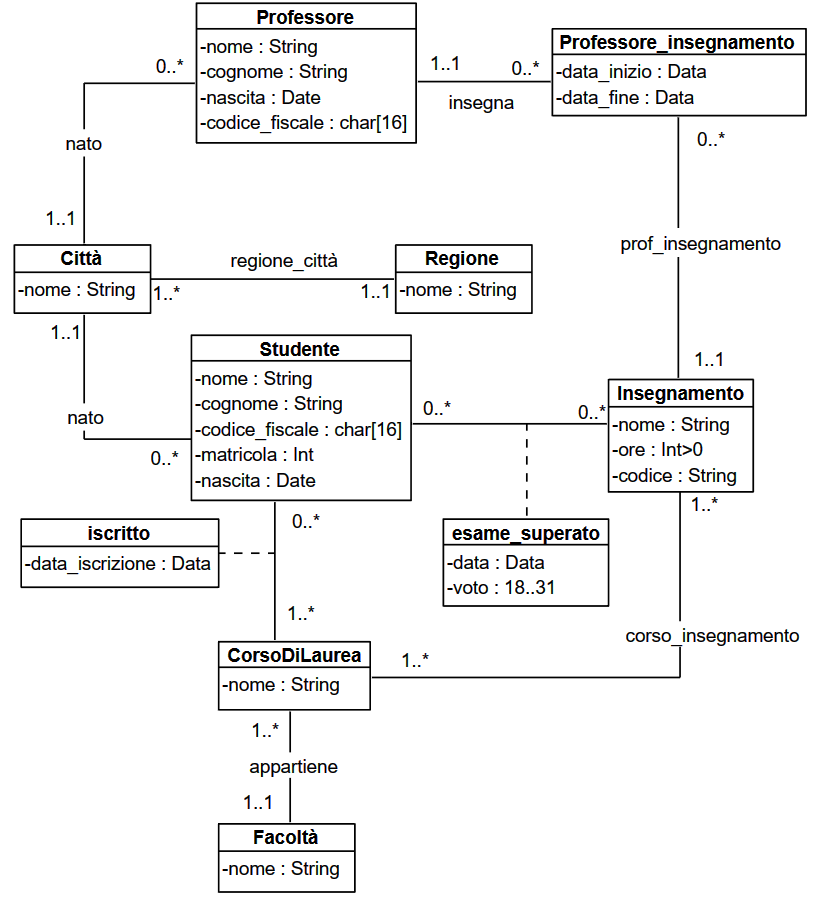
\includegraphics[width=\textwidth]{images/UML.png}


\end{document}

